\section{Quelle-Senke Beispiel}
Dieses minimalistische Beispiel soll die grundsätzliche Funktionsweise des Verifikationsalgorithmus und der BDD-Optimierung erläutern und demonstrieren, wie durch die Optimierung der Zustandsraum von Modellen reduziert werden kann.

Das System besteht aus zwei Komponenten:
Die Quelle hat einen Ausgang und gibt die Sequenz der natürlichen Zahlen modulo 10 zurück, also
\[ 0,1,2,3,4,5,6,7,8,9,0,1,2,\dots \]
Der Ausgang der Quelle ist mit der Eingabe der Senke verbunden.
Diese prüft, ob der Wert an ihrem Eingang kleiner als 12 ist und setzt dann den Ausgang auf den Wert 0, andernfalls auf 1.
Zu verifizieren ist in diesem Beispiel, dass der Ausgabewert der Senke stehts 0 ist.

Für den Kontrakt bietet sich also an zu spezifizieren, dass die Quelle stets Werte produziert, die kleiner als 10 sind.
Die Senke produziert für Werte kleiner 10 stets die Ausgabe 0, was sich ebenfalls als Kontrakt formulieren lässt.
Die resultierende GTL-Beschreibung sieht wie folgt aus:
\begin{lstlisting}[language=gtl]
model[scade] source("source_sink.scade","Source") {
  contract always outp < 10;
  init outp 9;
}

model[scade] sink("source_sink.scade","Sink") {
  init outp 0;
  contract always (inp < 10 => outp=0);
}

connect source.outp sink.inp;

verify {
  always sink.outp=0;
}
\end{lstlisting}
Das Kontrakt-Automaten System, dass sich aus dieser Beschreibung ergibt ist in Abbildung \ref{fig:source_sink_automata} gezeigt.

\begin{figure}[h]
  \centering
  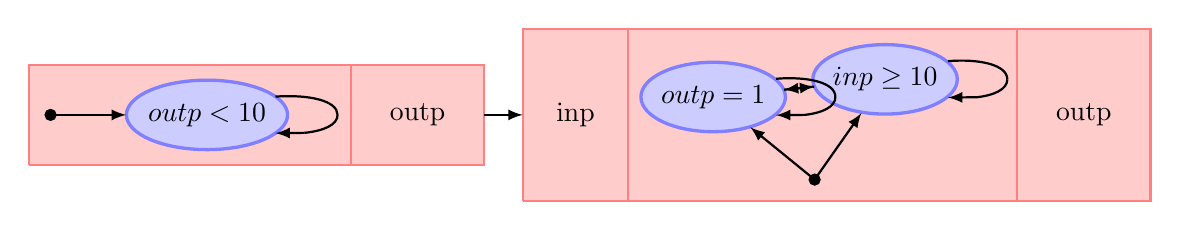
\begin{tikzpicture}
    \draw[color=red!50,fill=red!20,thick] (178.82bp,1.5bp) -- (216.82bp,1.5bp) -- (216.82bp,63.5bp) -- (178.82bp,63.5bp) -- (178.82bp,1.5bp);
\draw[color=red!50,fill=red!20,thick] (216.82bp,1.5bp) -- (356.82bp,1.5bp) -- (356.82bp,63.5bp) -- (216.82bp,63.5bp) -- (216.82bp,1.5bp);
\draw[color=red!50,fill=red!20,thick] (356.82bp,1.5bp) -- (404.82bp,1.5bp) -- (404.82bp,63.5bp) -- (356.82bp,63.5bp) -- (356.82bp,1.5bp);
\draw (197.82bp,32.5bp) node {inp};
\draw (380.82bp,32.5bp) node {outp};
\begin{scope}[shift={(220.375bp,6.2044999999999995bp)}]
\draw [color=blue!50,very thick,fill=blue!20](88.888bp,39.091bp) ellipse (25.99992bp and 12.49992bp);
\draw (88.888bp,39.091bp) node {$\begin{array}{c}inp\geq 10\end{array}$};
\draw [color=blue!50,very thick,fill=blue!20](27.0bp,32.748bp) ellipse (25.99992bp and 12.49992bp);
\draw (27.0bp,32.748bp) node {$\begin{array}{c}outp=1\end{array}$};
\draw [fill](63.529bp,3.0bp) ellipse (2.000016bp and 2.000016bp);
\draw [-,thick] (111.53bp,45.642bp) .. controls (122.82bp,46.548bp) and (132.89bp,44.365bp) .. (132.89bp,39.091bp);
\draw [-,thick] (132.89bp,39.091bp) .. controls (132.89bp,35.548bp) and (128.34bp,33.4bp) .. (121.93bp,32.646bp);
\draw [-,thick] (63.359bp,36.475bp) .. controls (63.134bp,36.452bp) and (62.909bp,36.429bp) .. (62.683bp,36.406bp);
\draw [-,thick] (52.53bp,35.365bp) .. controls (52.754bp,35.388bp) and (52.979bp,35.411bp) .. (53.205bp,35.434bp);
\draw [-,thick] (49.639bp,39.299bp) .. controls (60.929bp,40.205bp) and (71.0bp,38.022bp) .. (71.0bp,32.748bp);
\draw [-,thick] (71.0bp,32.748bp) .. controls (71.0bp,29.205bp) and (66.454bp,27.057bp) .. (60.046bp,26.304bp);
\draw [-,thick] (64.618bp,4.5508bp) .. controls (66.427bp,7.1253bp) and (70.259bp,12.578bp) .. (74.354bp,18.407bp);
\draw [-,thick] (61.959bp,4.2783bp) .. controls (59.405bp,6.3579bp) and (54.054bp,10.716bp) .. (48.288bp,15.411bp);
\draw [-latex,thick] (121.93bp,32.646bp) -- (111.53bp,32.541bp);
\draw [-latex,thick] (62.683bp,36.406bp) -- (52.471bp,35.359bp);
\draw [-latex,thick] (53.205bp,35.434bp) -- (63.417bp,36.481bp);
\draw [-latex,thick] (60.046bp,26.304bp) -- (49.639bp,26.198bp);
\draw [-latex,thick] (74.354bp,18.407bp) -- (80.338bp,26.923bp);
\draw [-latex,thick] (48.288bp,15.411bp) -- (40.394bp,21.84bp);
\end{scope}

\draw[color=red!50,fill=red!20,thick] (1.0bp,14.5bp) -- (117.0bp,14.5bp) -- (117.0bp,50.5bp) -- (1.0bp,50.5bp) -- (1.0bp,14.5bp);
\draw[color=red!50,fill=red!20,thick] (117.0bp,14.5bp) -- (165.0bp,14.5bp) -- (165.0bp,50.5bp) -- (117.0bp,50.5bp) -- (117.0bp,14.5bp);
\draw (141.0bp,32.5bp) node {outp};
\begin{scope}[shift={(5.840000000000003bp,19.0bp)}]
\draw [color=blue!50,very thick,fill=blue!20](59.321bp,13.5bp) ellipse (29.00016bp and 12.49992bp);
\draw (59.321bp,13.5bp) node {$\begin{array}{c}outp<10\end{array}$};
\draw [fill](3.0bp,13.5bp) ellipse (2.000016bp and 2.000016bp);
\draw [-,thick] (83.985bp,20.085bp) .. controls (95.848bp,20.898bp) and (106.32bp,18.703bp) .. (106.32bp,13.5bp);
\draw [-,thick] (106.32bp,13.5bp) .. controls (106.32bp,9.9229bp) and (101.37bp,7.7675bp) .. (94.422bp,7.0339bp);
\draw [-,thick] (4.8739bp,13.5bp) .. controls (7.6696bp,13.5bp) and (13.321bp,13.5bp) .. (19.967bp,13.5bp);
\draw [-latex,thick] (94.422bp,7.0339bp) -- (83.985bp,6.9148bp);
\draw [-latex,thick] (19.967bp,13.5bp) -- (30.196bp,13.5bp);
\end{scope}

\draw [-,thick] (165.0bp,32.5bp) .. controls (165.0bp,32.5bp) and (166.63bp,32.5bp) .. (168.78bp,32.5bp);
\draw [-latex,thick] (168.78bp,32.5bp) -- (178.82bp,32.5bp);


  \end{tikzpicture}
  \caption{Quelle-Senke Kontrakt-Automaten}
  \label{fig:source_sink_automata}
\end{figure}

Wenig erstaunlich ist nun das Ergebnis der Verifikation:
Da die BDD-Abstraktion die Bedingung $\mathit{outp}<10$ als eine Transition betrachtet, ist das resultierende Transitionssystem in der BDD-Verifikation bedeutend kleiner als in der C-Integration (Siehe Tabelle \ref{tab:source_sink_verifikation}).

\begin{table}
  \centering
  \begin{tabular}{|l|r|r|r|}
    \hline
    \textbf{Modus} & \textbf{Zustände} & \textbf{Transitionen} & \textbf{Speicherverbrauch}\\
    \hline
    Native & 25 & 49 & 4,653 MB\\
    BDD & 6 & 11 & 4,653 MB\\
    \hline
  \end{tabular}
  \caption{Quelle-Senke Verifikationsergebnisse}
  \label{tab:source_sink_verifikation}
\end{table}
\section{Mutex Beispiel}
Das Problem des gegenseitigen Ausschluss, besser bekannt unter der englischen Bezeichnung "`mutual exclusion"' oder kurz \emph{mutex} wurde erstmals 1965 von Edsger Dijkstra formalisiert~\cite{dijkstra_mutex}.
Zwei oder mehr Prozesse versuchen in diesem Problem, Zugriff auf eine Ressource zu erhalten, die aber nur einem Prozess zur Zeit zur Verfügung stehen darf.
Die Ressource kann hierbei beispielsweise ein Ausgabegerät sein, dass bei gleichzeitiger Benutzung fehlerhafte Ausgaben produziert, oder eine Speicherstelle, die inkonsistent beschrieben wird, wenn zwei Prozesse gleichzeitig auf sie schreiben.

Die Aufgabe ist nun, ein Protokoll zu entwerfen, wie die Prozesse sich die Ressource teilen können und trotzdem die folgenden Eigenschaften erfüllt sind:
\begin{itemize}
\item Die Ressource wird immer nur von einem oder keinem Prozess zur Zeit verwendet.
  Diese Eigenschaft stellt eine so genannte Sicherheitseigenschaft\footnote{engl. \emph{safety property}} dar, denn sie sagt aus, dass das System nie in einen unsicheren Zustand gerät.
\item Wenn ein Prozess die Ressource haben möchte, so wird er sie irgendwann auch erhalten.
  Diese Eigenschaft verhindert, dass man die Sicherheitseigenschaft einfach erfüllt, indem man die Ressource nie an einen Prozess vergibt.
  Es handelt sich hierbei um eine so genannte Lebendigkeitseigenschaft\footnote{engl. \emph{liveness property}}, denn sie sagt aus, dass das System immer "`am Leben"' bleibt, indem alle Prozesse bedient werden (kein Prozess muss ewig warten).
\end{itemize}
Die Prozesse können sich in einem von vier Zuständen befinden:
\begin{description}
\item[nc] In diesem Zustand benötigt der Prozess die Ressource nicht.
  Alle Prozesse starten in diesem Zustand.
\item[acq] Der Prozess würde die Ressource gerne nutzen, besitzt sie aber noch nicht.
  Kann ihm die Ressource gerade nicht zugeteilt werden, so muss er in diesem Zustand warten.
\item[cs] Die Ressource befindet sich nun im Besitz des Prozesses.
  Solange er mit der Ressource arbeiten muss, bleibt er in diesem Zustand.
\item[rel] Hier gibt der Prozess die Kontrolle über die Ressource wieder ab.
\end{description}
In diesem Beispiel soll das Problem wie folgt gelöst werden:
Ein Server ist für die Verwaltung der Ressource verantwortlich.
Die Prozesse oder Klienten sind mit ihm verbunden und stellen, sobald sie sich im Zustand \emph{acq} befinden, eine Anfrage an den Server.
Dieser muss nun entscheiden, wie er die Ressource vergibt.

Zunächst modellieren wir einen Prozess.
Ein Prozess kommuniziert seinen aktuellen Zustand über die Enum-Variable \emph{st} an den Server.
Seine Eingabe-Variable \emph{proceed} gibt an, ob es dem Prozess momentan erlaubt ist, die Ressource an sich zu nehmen.
\begin{lstlisting}[language=gtl,numbers=left]
model[none] client() {
  input bool proceed;
  output enum { nc, acq, cs, rel } st;
\end{lstlisting}
Am Anfang befindet sich der Prozess im Zustand \emph{nc}:
\begin{lstlisting}[language=gtl,numbers=left,firstnumber=last]
  init st 'nc;
\end{lstlisting}
Das Verhalten des Prozesses wird nun über eine Zustandsmaschine angegeben.
Der Prozess kann immer entweder im aktuellen Zustand verweilen, oder in den nächsten übergehen.
Der Übergang vom Zustand \emph{acq} zu \emph{cs} ist allerdings nur möglich, wenn die Variable \emph{proceed} gesetzt ist.
\begin{lstlisting}[language=gtl,numbers=left,firstnumber=last]
  automaton {
    init state nc {
      st = 'nc;
      transition acq;
      transition nc;
    }
    state acq {
      st = 'acq;
      transition[proceed] cs;
      transition[!proceed] acq;
    }
    state cs {
      st = 'cs;
      transition rel;
      transition cs;
    }
    state rel {
      st = 'rel;
      transition nc;
    }
  };
}
\end{lstlisting}
Der Server besitzt für jeden Prozess einen Eingang, der ihn über den aktuellen Zustand des Prozesses informiert.
Außerdem kann er jedem Prozess die Ressource zuteilen, indem er den entsprechenden Eintrag in dem \emph{procouts}-Array setzt.
\begin{lstlisting}[language=gtl,numbers=left,firstnumber=last]
model[none] server() {
  input enum { nc, acq, cs, rel }^3 procstates;
  output bool^3 procouts;
\end{lstlisting}
Am Anfang ist es allen Prozessen untersagt die Ressource zu besitzen:
\begin{lstlisting}[language=gtl,numbers=left,firstnumber=last]
  init procouts [false,false,false];
\end{lstlisting}
Danach gilt: Fordert der erste Prozess die Ressource an, so wird sie ihm genau dann überlassen, wenn sich Prozess zwei und drei nicht im kritischen Abschnitt befinden.
Das gleiche gilt symmetrisch für die anderen beiden Prozesse.
Gilt keiner der Fälle, so darf kein Prozess die Ressource besitzen.
\begin{lstlisting}[language=gtl,numbers=left,firstnumber=last]
  always (procstates[0] = 'acq
          and procstates[1] != 'cs
          and procstates[2] != 'cs
          and procouts = [true,false,false])
         or (procstates[0] != 'acq 
             and procstates[1] = 'acq
             and procstates[0] != 'cs
             and procstates[2] != 'cs
             and procouts = [false,true,false])
         or (procstates[0] != 'acq
             and procstates[1] != 'acq
             and procstates[2] = 'acq
             and procstates[0] != 'cs
             and procstates[1] != 'cs
             and procouts = [false,false,true])
         or (procouts = [false,false,false]);
}
\end{lstlisting}
Nun werden die definierten Modelle instanziiert, wobei drei Instanzen des Klienten und eine Instanz des Servers angelegt wird.
\begin{lstlisting}[language=gtl,numbers=left,firstnumber=last]
instance client c0;
instance client c1;
instance client c2;

instance server s;
\end{lstlisting}
Die Variablen der Instanzen müssen natürlich verbunden werden, damit eine Kommunikation stattfindet.
\begin{lstlisting}[language=gtl,numbers=left,firstnumber=last]
connect c0.st s.procstates[0];
connect c1.st s.procstates[1];
connect c2.st s.procstates[2];

connect s.procouts[0] c0.proceed;
connect s.procouts[1] c1.proceed;
connect s.procouts[2] c2.proceed;
\end{lstlisting}
Das Verifikationsziel ist die Sicherheitseigenschaft aus der Problem-Beschreibung:
Es ist immer nur maximal ein Prozess in seiner kritischen Sektion.
\begin{lstlisting}[language=gtl,numbers=left,firstnumber=last]
verify {
  always (c0.st = 'cs => !(c1.st = 'cs or c2.st = 'cs));
  always (c1.st = 'cs => !(c0.st = 'cs or c2.st = 'cs));
  always (c2.st = 'cs => !(c0.st = 'cs or c1.st = 'cs));
}
\end{lstlisting}
Tabelle \ref{tab:mutex_results} zeigt die Ergebnisse der erfolgreichen Verifikation.
Eine Verifikation mit der BDD-Optimierung ist im aktuellen Entwicklungsstadium des Tools noch nicht möglich.
\begin{table}
  \centering
  \begin{tabular}{|l|r|r|r|}
    \hline
    \textbf{Modus} & \textbf{Zustände} & \textbf{Transitionen} & \textbf{Speicherverbrauch}\\
    \hline
    Native & 11175 & 118773 & 5,337 MB\\
    \hline
  \end{tabular}
  \caption{Mutex Verifikationsergebnisse}
  \label{tab:mutex_results}
\end{table}

